\documentclass[11pt,a4paper]{article}
\usepackage[utf8]{inputenc}
\usepackage{amsmath}
\usepackage{amsfonts}
\usepackage{amssymb}
\usepackage{graphicx}

\title{D-optimal Designs for Logistic Regression using a Genetic Algorithm}
\author{Will Gertsch}


\usepackage{setspace}
\doublespacing

\begin{document}
\maketitle

\begin{abstract}
Logistic regression is a popular model for a binary outcome. While locally D-optimal designs can be found analytically for the case of a linear predictor, adding a quadratic term or constricting the design interval makes finding the optimal design more challenging. In most of these cases, there is no known analytical result. We use  a genetic algorithm to find locally D-optimal designs for linear and quadratic models on any design interval. We are able to confirm previous results and find new designs in several cases. 
\end{abstract}

\section{Introduction}
\section{Preliminaries}
\subsection{Logistic Regression}
Suppose we have a binary outcome modeled as $y_i \sim \text{Bernoulli}(p_i)$ for observations $i = 1, \dots, n$ and $0 \leq p_i < 1$. We can add a predictor $x_i$ into the model using the logit link function
$$
\log\left( \frac{p_i}{1-p_i}\right) = \eta_i
$$
where $\eta_i = \beta_0  + \beta_1 x_{i}$ or $\eta_i = \beta_0  + \beta_1 x_{i} + \beta_2 x_i^2$. Rearranging, we obtain an expression for the mean of $y_i$ given $\eta_i$
$$
p_i = \frac{e^{\eta_i}}{1+e^{\eta_i}}= \frac{1}{1+e^{-\eta_i}} 
$$

The information matrix for this model may be expressed as
$$
M(\beta) = \sum_{i=1}^k p_i (1-p_i) f(x_i) f(x_i)' = X'WX
$$
where $W$ is a diagonal weight matrix with entries $p_i (1-p_i)$. The design matrix $X$ has rows $f(x_i)' = (1, x_i)$ if $\eta_i$ is linear. If $\eta_i$ is quadratic, then $f(x_i)' = (1,x_i,x_i^2)$.
\subsection{Optimal Design}
The goal of optimal design is to find the optimal predictor values $x_1,\dots, x_k $ given a fixed number of observations $N$. Each design point $x_i$ is assigned $n_i$ observations such that $\sum_{i=1}^k n_i = N$. Alternatively, we may assign a weight $w_i$ to each $x_i$ to convey the same information. In this case, $\sum_{i=1}^k w_i = 1$ where $w_i = n_i/N$.

\par A design using weights be written as
$$
\xi =
\begin{pmatrix}
x_1 & \dots & x_k\\
w_1 & \dots & w_k
\end{pmatrix}
$$

The design $x_i$ implies a corresponding information matrix for the logistic regression model. Let
$$
M = M(\xi, \beta) = \sum_{i=1}^k w_ip_i (1-p_i) f(x_i) f(x_i)' = X'WX
$$
be the design and model implied information matrix where $W$ now has diagonal entries $w_i p_i (1-p_i)$.

The optimality of a particular design is determined by some function of the information matrix. It can be shown that the determinant of the information matrix is inversely proportional to the size of the confidence region for the parameters $\beta_0$, $\beta_1$, and $\beta_2$. Therefore, we may define a design as being optimal if it maximizes the determinant of the information matrix. This criterion is called D-optimality. Equivalently, we may minimize
$$
\Psi(M) = -\log(|M|)
$$

It can be shown that $\Psi(M)$ is a convex function of the design points $x_1, \dots, x_k$ and  the weights $w_1, \dots, w_k$. However, $\Psi(M)$ also depends on the parameters $\beta_0$, $\beta_1$, and $\beta_2$. This means that nominal values will need to be supplied for these parameters. Therefore, we may obtain a locally D-optimal design by first providing values for the parameters and then minimizing $\Psi(M)$.

To check if a design is locally D-optimal, we calculate the sensitivity function
$$
ch(x) = g(x) f(x)'M(\xi, \beta)^{-1} f(x) - p
$$
where $p$ is the number of parameters in the model and
$$
g(x) = \frac{\exp(\eta)}{(1+\exp(\eta))^2}
$$
The equivalence theorem says a design is locally D-optimal if and only if $ch(x) \leq 0 $ for all $x$ in the design interval with equality at the design points.


\subsection{Genetic Algorithm}
Finding a locally D-optimal design for the logistic model requires we optimize a function of several variables. This can be accomplished analytically for a linear $\eta$, but the complexity dramatically increases for a quadratic $\eta$ and requires a numerical solution. The objective function is complicated and changes between linear and quadratic models. Therefore, we should use an optimization algorithm that is gradient free. Additionally, we should use an algorithm that can incorporate constraints on the design space and require that the weight variables sum to 1.

The genetic algorithm (Holland, 1975) is a nature-inspired metaheuristic optimization algorithm. The algorithm mimics natural selection with the intended goal of ``evolving" a population of solution vectors towards an optimal value. Like other nature-inspired optimization algorithms, the genetic algorithm has the advantages of being gradient free, able to accommodate constraints, and able to escape local optimums. 

There are many variations on the genetic algorithm, but these algorithms usually contain the following three steps that are run every iteration of the algorithm. First, the \textit{crossover} operation combines two parent solutions to make two child solutions. Second, the \textit{mutation} operation randomly perturbs the child solutions. Finally, \textit{fitness} is assessed and the solution vectors that have the best objective function values move on to the next generation.

The following paragraphs detail the implementation of the genetic algorithm in PlatEMO. Let $N$ be the population size and let $D$ be the number of variables in the optimization problem. For simplicity, the description will assume $D=1$, but the process is eaily generalized to an arbritrary number of variables.

\begin{flushleft}
\textbf{Selection}
\end{flushleft}
The first step in the genetiec algorithm is to select the mating pool via tournament selection. $N$ paris are sampled with replacement from the population. The objective function values for eahc of these pairs is combared and the most opitmal of the pair is selected.

\begin{flushleft}
\textbf{Crossover}
\end{flushleft}
Once the mating pool has been selected, the two parents enter the crossover stage where genetic information is exchanged. This is done using the simulated binary crossover procedure (Deb et. al. 2007). This procedure will generate a probability distribution from which the child characteristics are drawn from.

First, $\mu$ is drawn from the uniform distribution on $(0,1)$. If $u \leq 0.5$, then set $\beta = 2\mu^{1/(d_c+1)}$. If $\mu > 0.5$, then set $\beta = (2-2\mu)^{-1/(d_c+1)}$. 

The $d_c$ parameter is the distribution index of the simulated binary crossover and is related to the variance of the child solutions from the parents. If $d_c$ is large, then the children will likely be close to the parents.  If $d_c$ is small, then the child solutions are more likely to be farther from the parents.

The $\beta$ calculated in this way is a spread factor defined as 
$$
\beta = \left| \frac{C_2 - C_1}{P_2 - P_1} \right|
$$
where $C_1, C_2$ are child values and $P_1, P_2$ are the parent values. Therefore $\beta$ measures the distance between children relative to the distance between parents.

Once $\beta$ has been found, the child solutions may be computed as
$$
C_1 = 0.5\left[(1+\beta)P_1 + (1-\beta)P_2 \right]
$$
and 
$$
C_2 = 0.5\left[(1-\beta)P_1 + (1+\beta)P_2 \right]
$$

Finally, this update is applied from probability $p_c$. In the implementation used by PlatEMO, additional steps are to set an expected number of crossovers for each pair of parents. On average, we should see $0.25 p_cD$ crossovers.

\begin{flushleft}
\textbf{Mutation}
\end{flushleft}
After crossover, each child solution is randomly perturbed. This helps the algorithm to better explore the objective space and hopefully escape local optima. This is acheived using a polnomial probabily distribution with mean at the current value and with variance equal to a function of $d_M$, the distribution index of mutation.



\begin{flushleft}
\textbf{Fitness}
\end{flushleft}
Once the crossover and mutation operations take place, there will be a population of size $2N$. The objective function is evaluated for each of these solutions and the best $N$ are chosen to move on to the next generation.



\section{Results}
The genetic algorithm was implemented using the PlatEMO framework in MATLAB. We used the built-in algorithm ``GA'' with default parameters ($p_C = 1, d_C = 20, p_M = 1, d_M = 20$). We found that running the algorithm for 100000 function evaluations with a swarm size of 1000 was able produce near optimal designs for every design we tried. 

When the optimal number of design points was unknown, we ran the algorithm once with 10 design points and then made a guess at the correct number of design points. The optimal number of design points was easy to guess after seeing the sensitivity plot.

\subsection{Linear $\eta$ on $(-\infty, \infty)$}
If $\eta_i = \beta_0 + \beta_1 x_i$ and the design interval is $(-\infty, \infty)$, it can be shown that the locally D-optimal design is equally weighted at $x_1$ and $x_2$ where
$$
x_1, x_2 = \frac{\pm 1.5434 - \beta_0}{\beta_1}
$$

For example, if $\beta_0 = 1$ and $\beta_1 = 1$ then the optimal design is
$$
\xi = \begin{pmatrix}
-1.5434 & 1.5434\\ 0.5 & 0.5
\end{pmatrix}
$$

The genetic algorithm was able to replicate this theoretical result. Table 1 shows designs for several nominal values of $\beta$ with the theoretical designs and the designs generated from the genetic algorithm. The algorithm is able to come very close to the theoretical result. Sensitivity plots confirm that the designs generated by the genetic algorithm are almost indistinguishable from the true optimum. Figure 1 shows one such sensitivity plot.
\begin{table}[ht]
\centering
\begin{tabular}{|c|c|c|}
\hline 
$\mathbf{\beta}$ & \textbf{Theoretical} & \textbf{GA} \\ 
\hline 
0,1 & $\begin{bmatrix}
-1.5434 & 1.5434\\ 0.5 & 0.5
\end{bmatrix}$  & $\begin{bmatrix}
-1.5452 & 1.5435\\ 0.5000 & 0.5000
\end{bmatrix}$ \\ 
\hline 
0.3,0.4 & $\begin{bmatrix}
-4.6085 & 3.1085\\ 0.5 & 0.5
\end{bmatrix}$  & $\begin{bmatrix}
-4.6091 & 3.1083\\ 0.5000 & 0.5000
\end{bmatrix}$ \\ 
\hline 
2,-5 & $\begin{bmatrix}
0.0913 & 0.7087\\ 0.5 & 0.5
\end{bmatrix}$  & $\begin{bmatrix}
0.0923 & 0.7109\\ 0.5000 & 0.5000
\end{bmatrix}$  \\ 
\hline
-4, 10 & $\begin{bmatrix}
0.2457 & 0.5543\\ 0.5 & 0.5
\end{bmatrix}$  & $\begin{bmatrix}
0.2475 & 0.5587\\ 0.5000 & 0.5000
\end{bmatrix}$\\
\hline 

\end{tabular} 
\caption{Locally D-optimal designs generated by the genetic algorithm compared to analytic solution.}
\end{table}

\begin{figure}
\centering
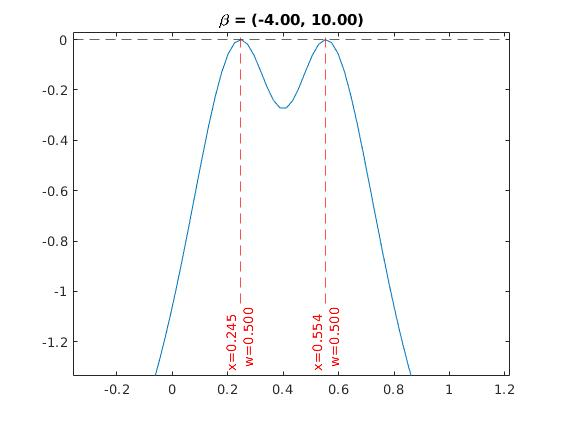
\includegraphics[scale=0.5]{figures/fig1.jpg}
\caption{Sensitivity function for design produced by genetic algorithm for a nominal $\beta$.}
\end{figure}

\subsection{Linear $\eta$ on other intervals}
The genetic algorithm can find designs on an arbitrary design interval $[a,b]$. In general, the optimal design will change from the design on $(-\infty, \infty)$ if any of the designs points is no longer included in the interval. Therefore, at least one of the two design points will likely be one of the bounds of the interval. Theoretical justifications for this phenomenon can be found in Sebastiani. 

Table 2 shows how the design interval affects the optimal design points. For example, if the interval excludes the global optimal point -1.543, then the optimal design will have one point at the bound of the design interval closest to that point. The other design point is also changed from $1.543$ to 1.796 to adjust for the change in the first point. All the designs remain equally weighted.

\begin{table}
\centering
\begin{tabular}{|c|c|c|c|c|c|}
\hline 
  & $[-\infty, \infty]$  & $[-1, \infty]$ & $[-\infty,1]$ & $[-1,1]$ & $[10, 20]$\\ 
\hline 
$x_1 (T)$ & -1.543 & -1 & -1.796 & -1  & ?\\ 
\hline 
$x_2 (T)$ & 1.543 & 1.796 & 1 & 1 & ?\\ 

\hline
$x_1 (GA)$ & -1.545 & -1 & -1.796 & -1 & $10$\\
\hline
$x_2 (GA)$ & 1.544 & 1.796 & 1 & 1 & $12$\\
\hline
\end{tabular}
\caption{Design points for locally D-optimal designs on several intervals for $\beta = (0,1)$ from theoretical and genetic algorithm approaches. ?: theoretical result not known.}
\end{table}

For the case when $a,b$ were both greater than the optimal design points on $(-\infty, \infty)$, there was no analytical result. However, the genetic algorithm was able to find an optimal design in this case. The last column of Table 2 shows optimal design on the interval $[10,20]$ and the sensitivity plot in Figure 2 confirms optimality.

\begin{figure}
\centering
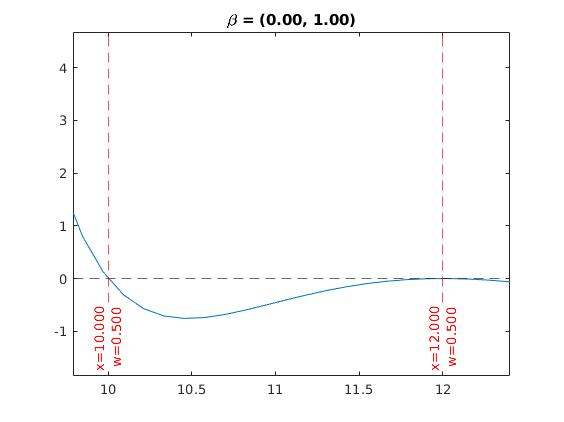
\includegraphics[scale=0.5]{figures/fig2.jpg}
\caption{Sensitivity plot for a design generated by the genetic algorithm on the design interval [10, 20].}
\end{figure}

\subsection{Quadratic $\eta$ on $(-\infty, \infty)$}
There are no analytic results for locally D-optimal designs when $\eta_i = \beta_0 + \beta_1 x_i + \beta_2 x_i^2$. However, Fornious was able to find locally D-optimal designs numerically for several nominal $\beta$. If $\beta_1 \neq 0$, then the design shifts along the design space. Therefore, the example nominal values have $\beta_1$ set at 0.

Table 3 compares the results from Fornious with the results from the genetic algorithm. The designs produced by the genetic algorithm are very close to the designs from Fornious and have sensitivity plots that indicate optimality. Some sets of nominal parameter values result in an optimal 3 point design while others have an optimal design with 4 points. Figure 3 shows the sensitivity plot for a 4 point design with $\beta = (2, 0, -0.1)$. Figure 4 shows a 3 point design for $\beta = (-2, 0, -4)$.
\begin{table}
\begin{flushleft}
\begin{tabular}{|c|c|c|}
\hline 
 Nominal values & Fornious & GA \\ 
\hline 
 $2,0,-0.1$ & 
$\begin{bmatrix}
-5.7185 & -2.7017  & 2.7017 & 5.7185\\
0.3138 & 0.1862 & 0.1862 & 0.3138
\end{bmatrix}$  & $\begin{bmatrix}
-5.7229 & -2.6945 & 2.7579 & 5.7229\\
0.3141 & 0.1894 & 0.1840 & 0.3126
\end{bmatrix}$\\ 
\hline 
 $2,0,-4$ & $\begin{bmatrix}
-0.9042 & -0.4272  & 0.4272 & 0.9042\\
0.3138 & 0.1862 & 0.1862 & 0.3138
\end{bmatrix}$  & $\begin{bmatrix}
-0.9051 & -0.4275  & 0.4272 & 0.9038\\
0.3139 & 0.1873 & 0.1850 & 0.3139
\end{bmatrix}$\\ 
\hline 
 $-2,0,-0.1$ & 
$\begin{bmatrix}
-3.9819 & 0.0000  & 3.9819\\
0.3333 & 0.3333 & 0.3333
\end{bmatrix}$   & $\begin{bmatrix}
-3.9818 & -0.0001  & 3.9813\\
0.3333 & 0.3333 & 0.3333
\end{bmatrix}$ \\ 
\hline 
 $-2,0,-4$ & 
$\begin{bmatrix}
-0.6296 & 0.0000  & 0.6296\\
0.3333 & 0.3333 & 0.3333
\end{bmatrix}$ & $\begin{bmatrix}[
-0.6295 & 0.0000  & 0.6296\\
0.3333 & 0.3333 & 0.3333
\end{bmatrix}$\\ 
\hline 
\end{tabular} 
\end{flushleft}

\caption{Designs for a quadratic $\eta$ from Fornious and the genetic algorithm.}
\end{table}

\begin{figure}
\centering
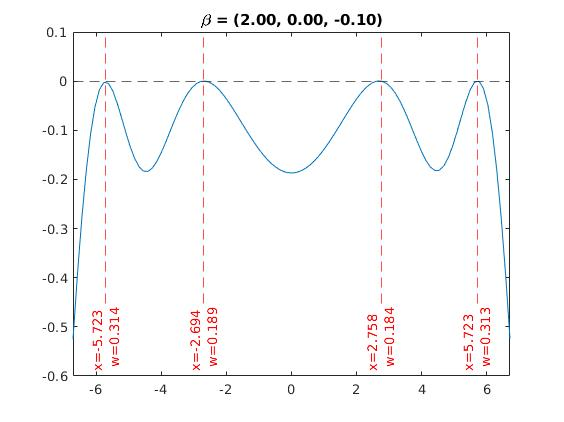
\includegraphics[scale=0.5]{figures/fig3.jpg}
\caption{Sensitivity plot for a 4 point design found for quadratic $\eta$ using the genetic algorithm.}
\end{figure}

\begin{figure}
\centering
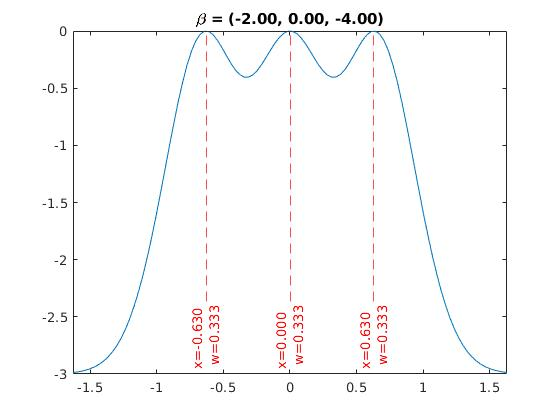
\includegraphics[scale=0.5]{figures/fig4.jpg}
\caption{Sensitivity plot for a 3 point design found for quadratic $\eta$ using the genetic algorithm.}
\end{figure}

The locally D-optimal designs for a quadratic $\eta$ have a few interesting features. First all designs are symmetric on the design space. This is easy to see when $\beta_1 = 0$, but also holds true when $\beta_1 \neq 0$. Secondly, the 3 point designs have equal weights at each design point. Finally,  the weights on each side of the symmetric 4 point designs sum to 1/2.

\section{Quadratic $\eta$ on other intervals}
There are many possible ways to restrict the design interval for the quadratic model. This is especially true when the locally D-optimal design on the unbounded interval has 4 points. To simplify the infinite number of nominal value and design interval combinations, we will restrict our focus on the nominal $\beta$ values of $(2, 0, -4)$ and $(-2, 0, -4)$ which give 4 and 3 point designs respectively. By modifying the design interval to include or not include the original optimal design points, we obtain insights that should generalize to other nominal values.

Recall that the locally D-optimal design for $\beta = (2,0,-4)$ on $(-\infty, \infty)$ has design points at $x_1=-0.9051, x_2=-0.4275, x_3=0.4272,$ and  $x_4=0.9038$. If the design interval is constructed such that $x_1$ and $x_4$ are not included, we get a 3 point equally weighted design with points at the bounds of the interval and at the axis of symmetry. Figure 5 shows the design when the interval is $[-0.5, 0.5]$. Restricting the interval to not include any of the original design points and placing the interval to be between $x_2$ and $x_3$ produces a similar design in Figure 6. We may also construct designs where the interval includes $x_3$ and $x_4$.  For the interval $[0,1]$, this produced an equally weighted 3 point design as can bee seen in figure 7.



\begin{figure}
\centering
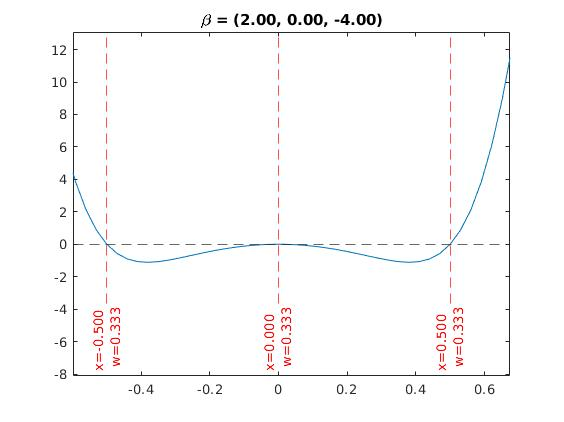
\includegraphics[scale=0.5]{figures/4pt_include2mid.jpg}
\caption{Sensitivity plot for a design on $[-0.5, 0.5]$ for a quadratic $\eta$.}
\end{figure}

\begin{figure}
\centering
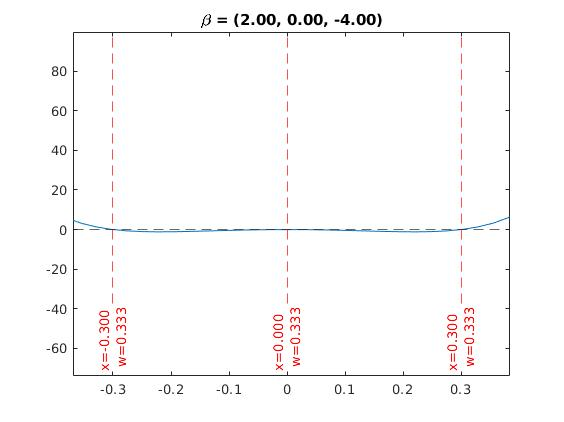
\includegraphics[scale=0.5]{figures/4pt_nonemid.jpg}
\caption{Sensitivity plot for a design on $[-0.3, 0.3]$ for a quadratic $\eta$.}
\end{figure}


\begin{figure}
\centering
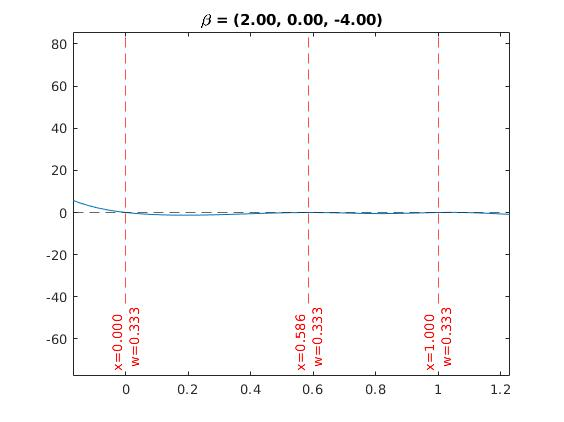
\includegraphics[scale=0.5]{figures/4pt_includeend2.jpg}
\caption{Sensitivity plot for a design on $[0,1]$ for a quadratic $\eta$.}
\end{figure}

For the originally 3 point design with $\beta = (-2, 0, -4)$, the results are very similar. Recall the optimal design for these nominal values was equally weighted at $x_1=-0.6295$, $x_2 = 0$,  and $x_3 = 0.6296$. If $x_2, x_3$ are included in the design interval, the result is an equally weighted 3 point design. Figure 8 shows the optimal design on the interval $[0, 1]$.

\begin{figure}
\centering
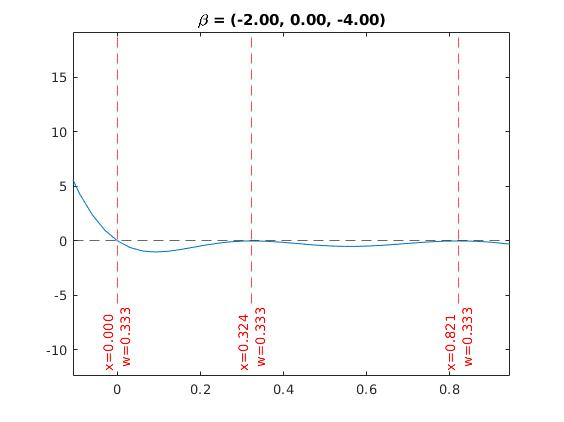
\includegraphics[scale=0.5]{figures/3pt_2include.jpg}
\caption{Sensitivity plot for a design on $[0,1]$ for a quadratic $\eta$.}
\end{figure}

Unfortunately, not all designs have a sensitivity plot that can easily plotted. The genetic algorithm still finds the design but it is difficult to judge from the plot whether the design is truly optimal. For example, Figure 9 shows the plot for $\beta = (-2, 0, -4)$ when the design interval is $[1,2]$. The sensitivity function at the design points is close to zero, but most of the curve is also very close to zero.


\begin{figure}
\centering
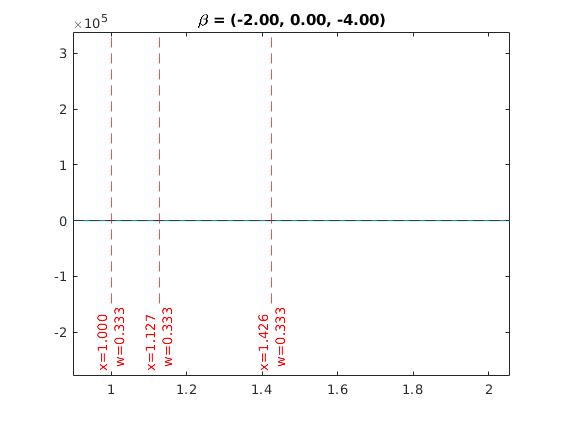
\includegraphics[scale=0.5]{figures/3pt_noneend.jpg}
\caption{Sensitivity plot for a design on $[1,2]$ for a quadratic $\eta$.}
\end{figure}




\section{Applications}
\section{Conclusions}
In this paper, we find locally D-optimal designs for linear and quadratic logistic regression using a genetic algorithm. We confirm existing analytical results for the linear model on any design interval. Additionally, we find a new design in the case when the design interval does not include the original optimal design points on the unbounded interval. Finally, we confirm previous results for a quadratic model and find new designs for a bounded design interval.

 Previous results depend on a variety of analytic and numeric methods to find the same designs. The advantage of our approach is that the genetic algorithm is a single method for finding optimal designs. This makes it easy for an investigator to change design parameters and find optimal designs for multiple scenarios.
 
Our approach can be extended to other design problems for the logistic regression model. This paper considered locally D-optimal designs, but future work may consider A, E, and G optimal designs. The logit link function may also be exchanged for other link functions. An extension to fractional polynomials (Royston \& Altman, 1994) may also be possible.
 
 
\section{References}
\section{Appendix}
\end{document}